\documentclass{standalone}
\usepackage{tikz}
\usepackage{ctex,siunitx}
\usepackage{tkz-euclide}
\usepackage{amsmath}
\usetikzlibrary{patterns, calc}
\usetikzlibrary {decorations.pathmorphing, decorations.pathreplacing, decorations.shapes,}
\begin{document}
\small
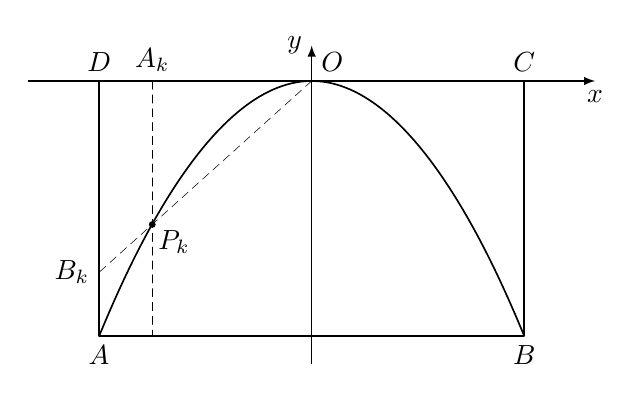
\begin{tikzpicture}[>=latex,scale=0.9]
  \draw[thin,->](-4,0)--(4,0)node[below]{$x$};
  \draw[thin,->](0,-4)--(0,0.5)node[left]{$y$};
  \tkzDefPoints{0/0/O,-3/-3.6/A,3/-3.6/B,3/0/C,-3/0/D,-3/-2.7/Bk,-2.25/0/Ak,-2.25/-3.6/AK}
  \tkzInterLL(Ak,AK)(O,Bk)\tkzGetPoint{Pk}
  \tkzDrawPolygon[semithick](A,B,C,D)
  \tkzDrawSegments[densely dashed](O,Bk Ak,AK)
  \draw[semithick](A)parabola bend (O) (B);
  \tkzDrawPoints[fill=black](Pk)
  \tkzLabelPoints[below](A,B)
  \tkzLabelPoints[above](C,D)
  \tkzLabelPoint[above](Ak){$A_k$}
  \tkzLabelPoint[left](Bk){$B_k$}
  \tkzLabelPoint[below right,inner sep=2pt](Pk){$P_k$}
  \tkzLabelPoints[above right](O)
\end{tikzpicture}
\end{document}